% report.tex for DA project

\documentclass{article}
\usepackage[utf8]{inputenc}
\usepackage{graphicx}


\title{Conway, Arkansas Airport - Temperature/Dewpoint Analysis}
\author{John Singel}\date{May 11, 2021}

\begin{document}

\maketitle

\section{Abstract}
This report uses a Python program to analyze temperature/dewpoint spreads from the Conway, Arkansas airport. When the spread is less than 2 degrees Celsius, the likelihood is that fog may form.

\section{Introduction}
In aviation there is an old saying: 'An excellent pilot is one who uses his excellent brain so that he does not have to use his excellent skills.' For over a century, now, aviators have relied on mnemonics and other devices to recall important information in a timely manner. These devices span from systems knowledge to preflight planning. One handy weather tool is the knowledge that when the temperature and dew point difference is two degrees Celsius or less, the chance of fog forming is high. This knowledge, in turn, will spur the aviator to plan for alternates and contingencies.

\section{Analysis}

\section{Conclusion}
\begin{figure}[h]
\begin{center}
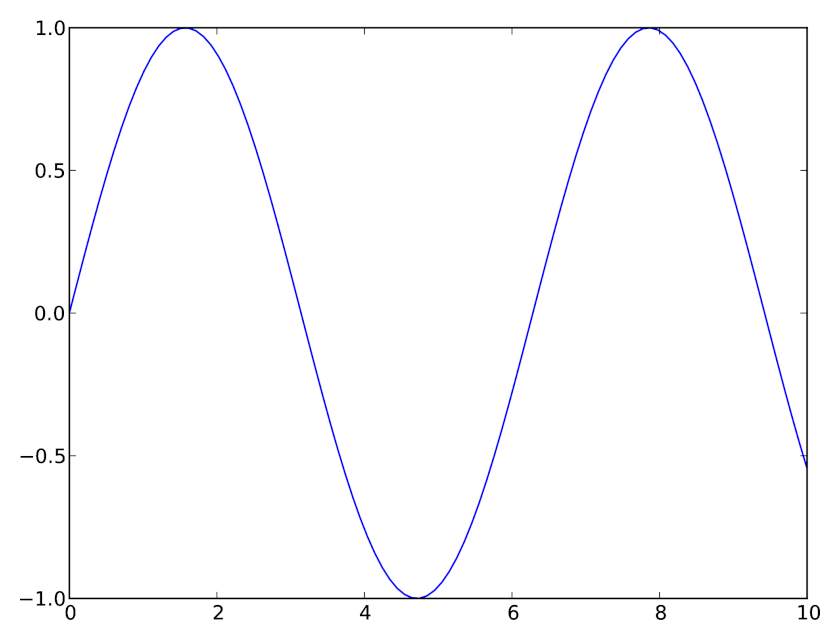
\includegraphics[width=0.5\textwidth]{fig3-1.png}
\end{center}
\caption{Graph of the sine wave}
\label{fig: 3-1}
\end{figure}

\subsection{How to use labels}
When referring to an item previously lableled, use the name of the label. For example: Figure  \ref{fig: 3-1}

$\alpha\lambda\lambda  \Gamma\rho\epsilon\epsilon\kappa$

\end{document}

